\section{Begrepp och systemöversikt}
\label{sec:begrepp och systemöversikt}

\begin{figure}
	\centering
	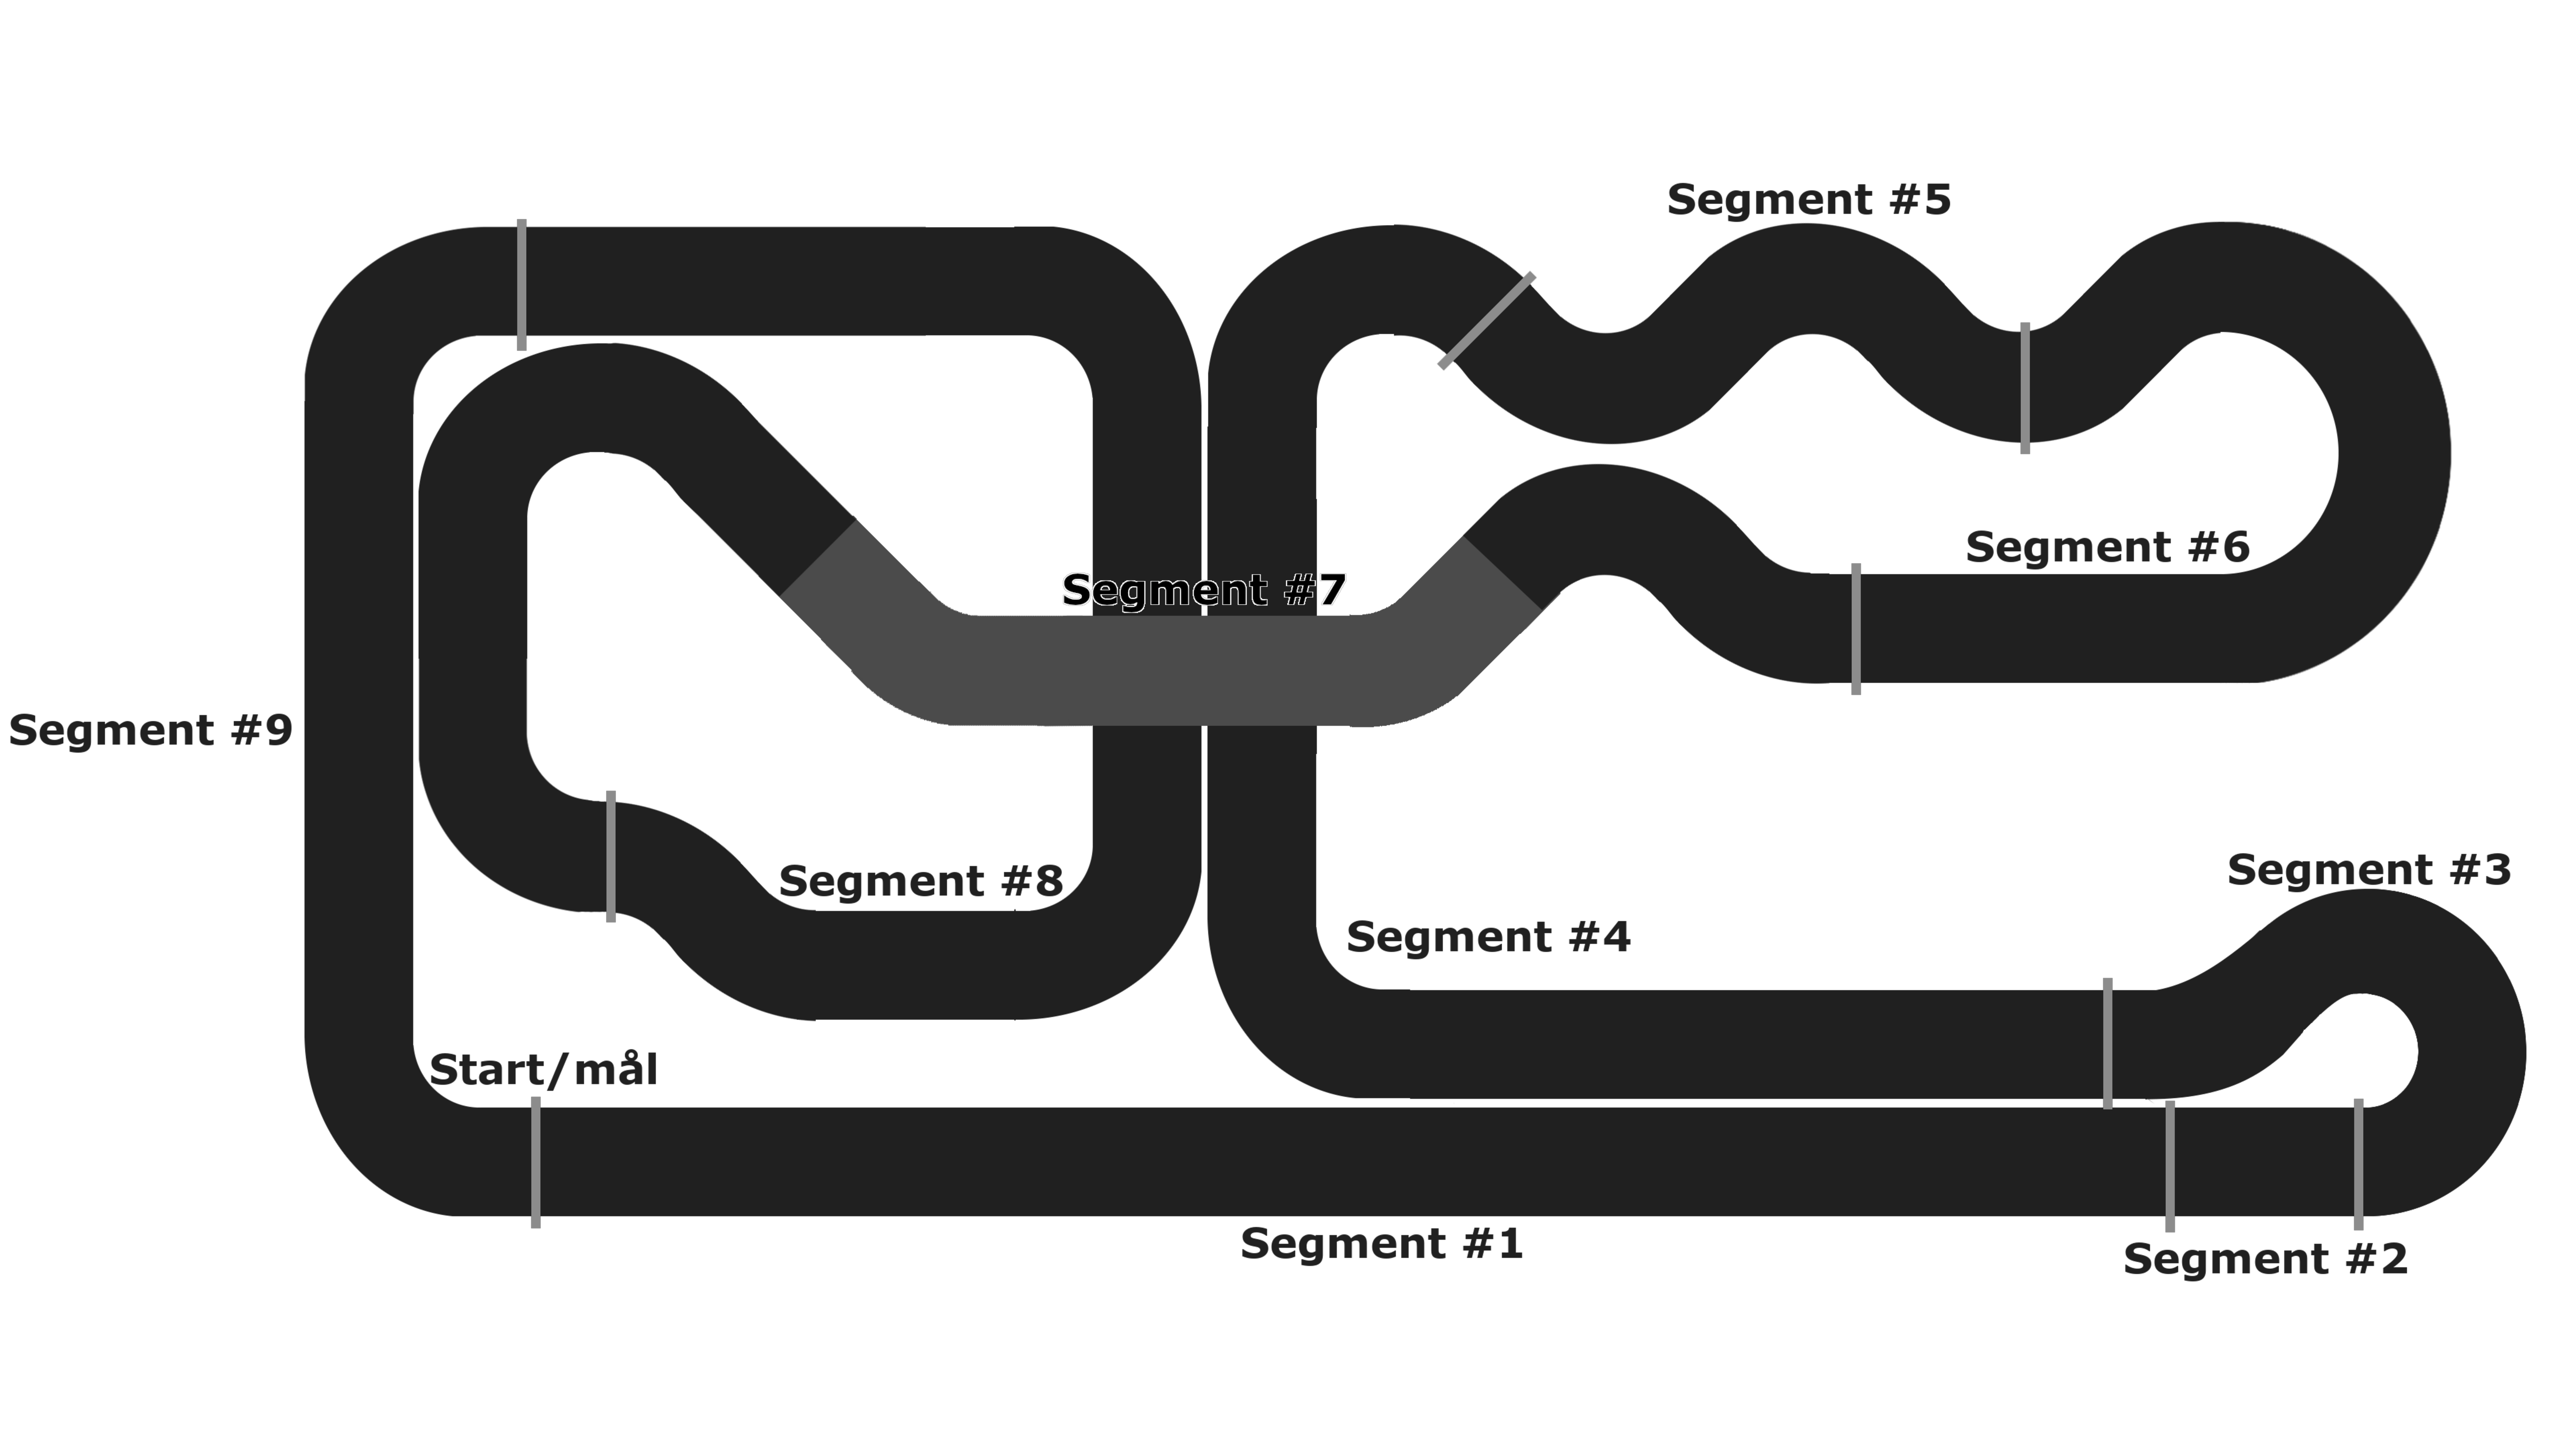
\includegraphics[width=\linewidth] {Figures/BanaModell}
	\caption{En modell av bilbanan.}
	\label{fig:bilbanan}
\end{figure} 

Runt om bilbanan finns nio givare (se Figur~\ref{fig:bilbanan}) som skickar en
signal när en bil passerar under dem. En av givarna kallas målgivaren vars
signal går att skilja från övriga givare och således passar som en markör för
när ett nytt varv inleds.  Givarna delar in banan i nio delar, kallade segment.
Dessa segment har i sin tur delats in i mindre delsegment. För vardera bana och
delsegment har ett värde på en \emph{spänningsparameter} tagits fram. Detta
värde varierar dels eftersom bilarna vid olika delar av banan behöver olika
mycket spänningstillförsel för samma hastighet och dels eftersom bilarna vid
vissa delar av banan inte kan åka lika snabbt som vid andra delar av banan för
att inte riskera att åka av.

För att anpassa efter olika bilars köregenskaper (vikt, motor, magnetstyrka och
så vidare) används en variabel kallad bilens \emph{konstant}. Konstanten tas
fram av systemet vid uppstart, justeras kontinuerligt under hela körningen och
är oberoende från tidigare körningar. Spänningen som skickas till banan
fås genom att multiplicera tidigare nämnda spänningsparameter med bilens
konstant.

% Centralt för systemet är den karta som beskrivs ovan samt en
% modifierare som beror på köregenskaperna för den nuvarande bilen. Det
% modifierande värdet kallas bilens \emph{konstant}. Denna konstant varierar
% beroende på hur mycket spänning en viss bil behöver för att nå en viss
% hastighet. Konstanten anpassas under körningens gång ytterligare beroende på
% bilens varvtid jämfört med referenstiden.

\subsection{Display}

Förutom bilbanan finns även en display. Innan körningen används den för att
välja vilka banor som ska köras, om de ska köras manuellt eller autonomt och
vilken referenstid som ska köras mot. Under körningen visas i realtid det
gaspådrag som skickas till banan och efter körningen visas varvtiderna och den
genomsnittliga tiden per segment, båda för vardera bil.

\subsection{Kommunikation}

För att rita objekt på displayen finns hjälpfunktioner liknande ett API som
matchar displayens tekniska specifikation, se bilaga. Hjälpfunktionerna beskrivs
i sin helhet i Appendix~\ref{app:funktioner och filer:display}.

För att reagera på knapptryck på displayen kan displayen instrueras att flytta
hela sitt interna minne (där information om bland annat knapptryck finns) till
ett minne som delas med styrdatorn. Detta minne kan sedan läsas av och systemet
kan agera utifrån händelserna som har skett.

% \begin{itemize}
% 
% 	\item \texttt{car.num} - Om bilen är på bana ett eller två.
% 	\item \texttt{car.running} - Om bilen körs eller inte.
% 	\item \texttt{car.stopping} - Om bilen för tillfället letar efter ett ställe att stanna på.
% 	\item \texttt{car.stopped} - Om bilen har hittat ett ställe att stanna på.
% 	\item \texttt{car.automatic} - Om bilen ska köras autonomt.
% 	\item \texttt{car.segment} - Bilens nuvarande segment.
% 	\item \texttt{car.lap} - Bilens nuvarande varv.
% 	\item \texttt{car.lap\_times} - En lista över bilens varvtider.
% 	\item \texttt{car.seg\_times} - En matris över bilens segmentstider per varv.
% 	\item \texttt{car.position} - Bilens position i meter efter målgivaren.
% 	\item \texttt{car.pos\_at} - En lista över hur långt det är kvar till målgivaren från de olika segmenten.
% 	\item \texttt{car.seg\_len} - En lista över längden för varje segment.
% 	\item \texttt{car.percents} - En lista över hur stor andel av varvtiden varje segment förväntas ta.
% 	\item \texttt{car.map} - Kartan över alla subsegment och önskad spänningstillförsel.
% 	\item \texttt{car.miss\_probability} - Sannolikheten att bilen vid en given givare inte får en signal. Används för att testa krav 3.
% 	\item \texttt{car.constant} - Multipliceras med den önskade spänningstillförseln för att
% 		kompensera för olika bilars olika påverkan av samma spänningstillförsel.
% 
% \end{itemize}
% 
% 
% Utöver dessa värden sparas ett antal värden för själva systemet.
% 
% \begin{itemize}
% 
% 	\item \texttt{display.data} - En kö av kommandon som ska skickas till displayen.
% 	\item \texttt{bootN.status} - Om den så kallade ''bootstrapen'' är aktiv för bana N. Se \ref{sec:systembeskrivning:uppstart}
% 	\item \texttt{bootN.time} - Den tid som passerat sedan förra gången ''bootstrapen'' höjde \texttt{car.constant} för bana N. Se 
% 	\ref{sec:systembeskrivning:uppstart}
% 	\item \texttt{halt} - Om någon av bilarna åkt av och användaren valt att avbryta körningen.
% 	\item \texttt{t} - Hur lång tid den nuvarande programcykeln tagit.
% 	\item \texttt{highToc} - Längden på den längsta programcykeln. Används för att kontrollera krav 31.
% 
% \end{itemize}
